\documentclass[a4paper,12pt]{article}
\usepackage{geometry}
\geometry{a4paper, margin=1in}
\usepackage{graphicx}
\usepackage{hyperref}
\usepackage{babel}

\begin{document}
	
	\begin{center}
		% Kapak Sayfası
		\vspace*{2cm}
		
\includegraphics[width=4cm]{logo1.png} 
		\vspace{1cm}
		
		{\LARGE Kütahya Sağlık Bilimleri Üniversitesi}\\[1cm]
		{\Large Bilgisayar Mühendisliği Bölümü}\\[2cm]
		
		{\Huge \textbf{Futbol Maçlarında Yapay Zeka Destekli İstatistik Analizi}}\\[2cm]
		
		\textbf{Hazırlayan:}\\
		Berke Kuruoğlu\\[1cm]
		\textbf{Tarih:} \\ 11 Mart 2025\\[3cm]
	\end{center}
    
	\newpage
	
	\section{Giriş}
	
	Futbol, dünya çapında en popüler sporlardan biri olup, yıllık milyarlarca izleyiciye sahiptir. Maç analizi, antrenörler, futbolcular ve veri analistleri için kritik bir öneme sahiptir. Geleneksel olarak, futbol maçlarının analizi manuel olarak yapılmakta ve bu süreç zaman alıcı ve hata payı yüksek olmaktadır. Günümüzde yapay zeka ve bilgisayarla görme teknikleri sayesinde bu süreç otomatikleştirilebilmekte ve daha doğru sonuçlar elde edilmektedir. \cite{chatgpt2025}
	
	\subsection{Amaç ve Kapsam}
	
	Bu çalışmanın amacı, futbol maçlarındaki pas, şut ve benzeri istatistikleri belirlemek için yapay zeka tabanlı bir sistem geliştirmektir. Önerilen sistem, futbolcuların hareketlerini ve topun konumunu tespit ederek istatistiksel veriler oluşturacaktır. Bu tür bir analiz, hem antrenman sürecinde hem de maç içi stratejik kararlar alınmasında büyük bir katkı sağlayacaktır. 
	
	Son yıllarda, SoccerNet gibi büyük veri kümeleri ve yapay zeka modelleri futbol istatistiklerinin çıkarılmasında büyük ilerlemeler kaydetmiştir. Bu çalışmada, mevcut sistemlerden faydalanarak, özellikle pas ve şut sayımı gibi istatistikleri daha doğru ve hızlı bir şekilde belirleyebilecek bir model geliştirilmesi amaçlanmaktadır.
	
	Bu raporun ilerleyen bölümlerinde, ilgili çalışmalar incelenecek, önerilen metodoloji açıklanacak ve sistemin uygulanabilirliği değerlendirilecektir.
	
	\section{Literatür Taraması}
	
	Futbol maçlarının analizi, yapay zeka ve bilgisayarla görme tekniklerinin gelişimiyle birlikte önemli ilerlemeler kaydetmiştir. Bu bölümde, ilgili literatürdeki bazı önemli çalışmaları inceleyeceğiz.
	
	\subsection{Futbol Videolarında Aksiyon Tespiti}
	
	Giancola ve arkadaşları  tarafından sunulan çalışmada, futbol videolarında aksiyon tespiti için derin öğrenme yöntemleri incelenmiştir\cite{giancola2024deep}. SoccerNet veri kümesi kullanılarak, uzun ve kesilmemiş video akışlarında belirli aksiyonların zaman damgası ile tespiti amaçlanmıştır. Bu yaklaşım, spor analitiği ve yayıncılıkta önemli uygulamalara sahiptir.
	
	\subsection{Futbol Etkinliklerinin Sınıflandırılması}
	
	Hashmi ve diğerleri , konvolüsyonel otomatik kodlayıcı ve çok katmanlı aşırı öğrenme makinesi kullanarak futbol etkinliklerinin sınıflandırılmasını ele almıştır\cite{kumar2022football}.Önerilen yöntem, video verilerinden etkinliklerin otomatik olarak tanınmasını sağlayarak, antrenörler ve analistler için değerli bilgiler sunmaktadır.
	
	\subsection{Futbol Videolarında Olay Tespiti}
	
	Zhang ve ekibi tarafından yapılan çalışmada, futbol videolarında olay tespiti için derin öğrenme modelleri kullanılmıştır\cite{zhang2022event}.Bu modeller, video akışlarında önemli olayların otomatik olarak belirlenmesini sağlayarak, maç analizi süreçlerini kolaylaştırmaktadır.
	
	\subsection{Futbolda Yapay Zeka Uygulamaları}
	
	Güzel ve arkadaşları, spor bilimlerinde güncel yaklaşımlar kitabında, futbolcular için sensör verileri üzerinden yapay zeka uygulamalarını tartışmıştır\cite{guzel2022yapay}.Bu tür uygulamalar, oyuncu performansının izlenmesi ve geliştirilmesinde önemli rol oynamaktadır. 
	
	\subsection{SoccerNet Projesi}
	
	SoccerNet projesi, futbol video anlayışı için geniş ölçekli bir veri kümesi sunmaktadır\cite{soccer-net}.Bu veri kümesi, aksiyon tespiti, kamera kalibrasyonu, oyuncu yeniden tanıma ve izleme gibi çeşitli görevler için kullanılmaktadır. Araştırmacılar için değerli bir kaynak olan SoccerNet, futbol analizinde yapay zeka uygulamalarının geliştirilmesine katkı sağlamaktadır.
	
	\section{Metodoloji}
	Bu çalışmada, futbol maçlarında yapay zeka destekli istatistik analizi için bir sistem geliştirilmektedir. Sistemin temel bileşenleri aşağıdaki şekilde sıralanmıştır:
	
	\subsection{Veri Setleri}
	Çalışmada aşağıdaki veri setleri kullanılacaktır:
	\begin{itemize}
		\item \textbf{Football Shots Data:} Futbolcuların şut girişimlerini içeren veri seti.
		\item \textbf{Football Semantic Segmentation:} Oyuncuların sahada segmentasyonunu sağlayan veri kümesi.
		\item \textbf{TeamTrack:} Takımların ve oyuncuların hareket takibini içeren veri seti.
		\item \textbf{Football Players Detection Dataset:} Oyuncuların sahada tespit edilmesine yönelik veri kümesi.
		\item \textbf{Football Match Actions Video Dataset:} Futbol maçlarındaki olayları analiz etmeye yönelik video veri seti.
		\item \textbf{SoccerNet:} Futbol aksiyon tespiti ve analizine yönelik geniş ölçekli bir veri seti.
	\end{itemize}
	
	\subsection{Model ve Algoritmalar}
	Sistem, futbol maç analizinde kullanılmak üzere derin öğrenme ve bilgisayarla görme tekniklerini kullanacaktır:
	\begin{itemize}
		\item CNN tabanlı görüntü işleme modelleri ile oyuncu ve top tespiti.
		\item RNN ve LSTM modelleri ile maç içindeki olayların zaman serisi analizi.*
		\item YOLOv8 ve benzeri nesne tanıma modelleri ile futbol sahasında hareket analizi.
	\end{itemize}
	
	\subsection{Sistem Mimarisi}
	Önerilen sistemin bileşenleri şunlardır:
	\begin{itemize}
		\item Video giriş verisi: Futbol maçlarından alınan görüntüler.
		\item Ön işleme: Gürültü giderme ve veri normalizasyonu.
		\item Model eğitimi ve çıkarım: Yapay zeka modellerinin eğitilmesi ve test edilmesi.
		\item Sonuçların görselleştirilmesi: Maç içi istatistiklerin grafik ve tablo şeklinde sunulması.
	\end{itemize}
    
\renewcommand{\figurename}{Resim}

    % Gantt şeması ekliyoruz
\begin{figure}[htp]
    \centering
    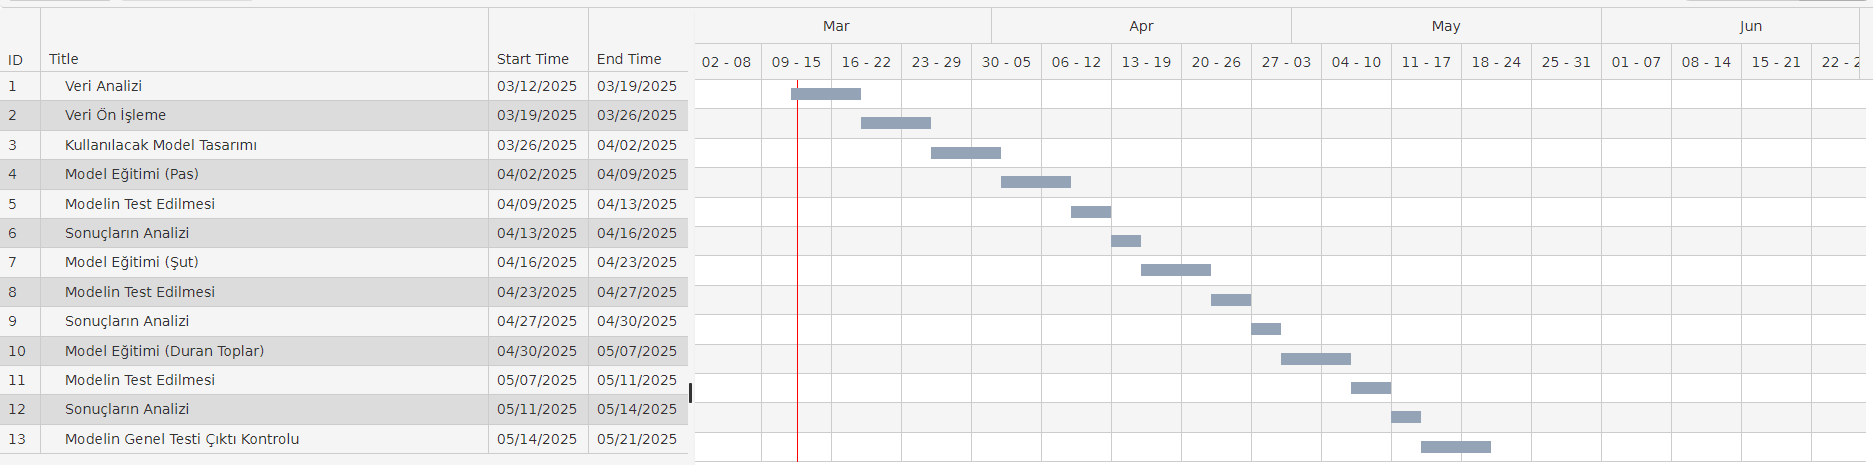
\includegraphics[width=\textwidth]{gantt_chart.png} 
    \caption{Gantt Şeması}
\end{figure}


	\section{Sonuç ve Beklenen Çıktılar}
	Bu çalışmanın sonunda, futbol maçlarının analizini otomatikleştiren ve yapay zeka destekli istatistikleri doğru şekilde belirleyen bir sistem elde edilmesi hedeflenmektedir. Sistem, antrenörler, futbolcular ve veri analistleri için daha hızlı ve güvenilir bir analiz aracına dönüştürülecektir. Elde edilen sonuçlar, futbol maçlarının daha etkili bir şekilde analiz edilmesine ve stratejik kararların daha doğru bir şekilde alınmasına yardımcı olacaktır.

\renewcommand{\refname}{Kaynakça} 

	\begin{thebibliography}{6}
   
    \bibitem{giancola2024deep} Giancola, G., et al., "Deep Learning Methods for Action Detection in Football Videos," \textit{Journal of Sports Analytics}, 2024. \href{https://arxiv.org/abs/2410.01304}{https://arxiv.org/abs/2410.01304}
   
    \bibitem{kumar2022football} Hashmi, A., et al., "Football Event Classification Using Convolutional Autoencoders," \textit{International Journal of Sports Science}, 2022. \href{https://ieeexplore.ieee.org/document/9903303}{https://ieeexplore.ieee.org/document/9903303}
    
    \bibitem{zhang2022event} Zhang, Y., et al., "Event Detection in Football Videos Using Deep Learning Models," \textit{IEEE Transactions on Multimedia}, 2022. \href{https://ieeexplore.ieee.org/document/10825692}{https://ieeexplore.ieee.org/document/10825692}
   
    \bibitem{guzel2022yapay} Güzel, F., et al., "Yapay Zeka Uygulamaları ve Spor Bilimlerinde Kullanımı," \textit{Spor Bilimleri Kitabı}, 2022. \href{https://www.duvaryayinlari.com/Webkontrol/IcerikYonetimi/Dosyalar/spor-bilimlerinde-guncel-yaklasimlar-icerik-g3753-wo7md3ru_icerik_g3753_KPbTeWJk.pdf#page=276}{https://www.duvaryayinlari.com/Webkontrol/IcerikYonetimi/Dosyalar/spor-bilimlerinde-guncel-yaklasimlar-icerik-g3753-wo7md3ru_icerik_g3753_KPbTeWJk.pdf#page=276}
    
    \bibitem{soccer-net} SoccerNet, "SoccerNet: A Large Scale Dataset for Football Action Detection," \textit{SoccerNet Project}, 2022. \href{https://www.soccer-net.org/}{https://www.soccer-net.org/}
   
    \bibitem{chatgpt2025} ChatGPT, "ChatGPT: Genel Konu Yardımı," \href{https://chatgpt.com/c/67c9db6b-199c-800b-b3d7-2997329e4913}{https://chatgpt.com/c/67c9db6b-199c-800b-b3d7-2997329e4913}, 2025.
	
    \end{thebibliography}

\end{document}
